\documentclass[11pt]{article}

\usepackage[utf8]{inputenc}
\usepackage[spanish]{babel}

%Package to generate latin text (Only for testing)
\usepackage{lipsum}

\usepackage{amsmath}
\usepackage{amsfonts}
\usepackage{amssymb}
%AMS packages for mathematical symbols

%package to include pictures and images
\usepackage{graphicx}

%Package to setup page layout
\usepackage[margin=1in, includefoot, includehead]{geometry}

%Uses hyperlinks in PDF (optional)
\usepackage[hidelinks, plainpages=false, pdfpagelabels=true]{hyperref}

%Header and Footer Stuff
\usepackage{fancyhdr}
\pagestyle{fancy}
\fancyhead{}
\fancyfoot{}
\fancyhead[R]{\myTitle}
\fancyfoot[L]{Eder Omar Zúñiga Zavala}
\fancyfoot[R]{\thepage}
\renewcommand{\footrulewidth}{1pt}

\usepackage{csquotes}
\usepackage[backend=biber,style=apa]{biblatex}
\addbibresource{ochoarticulosbibliografias.bib}
\addbibresource{fuentes_web.bib}

\setlength{\headheight}{14pt}



% Document Variables 
\newcommand{\myTitle}{Reporte de lectura analítica}
\newcommand{\myName}{eder omar zúñiga zavala}
\vspace{2cm}
\newcommand{\myClass}{Fundamentos de Inteligencia Artificial}
\newcommand{\myTecher}{DR. SAID POLANCO MARTAGÓN}
\newcommand{\myDate}{\today}



\usepackage{float}
\usepackage{booktabs}
\usepackage{tabularx}
\usepackage{array}
\usepackage{ragged2e}
\usepackage[table]{xcolor}

%Document Start
\begin{document}

\begin{titlepage}
	\begin{center}
		
\includegraphics[scale=0.75]{img/logo.png}\\
		[0.25in] 
		\huge{\textbf{Universidad Politécnica \\de Victoria}} \\
		[0.25in] 
		
		\textbf{\Large{Instituto de Ingeniería y Tecnología}}\\
		\Large{Ingeniería en tecnologías de la información e innovación}\\
		[1in]

		\line(1,0){400}\\
		[2mm]
		\textsc{\Large{\myTitle}} \\
		\line(1,0){400} \\
		[1in]
	\end{center}
	\begin{center}
		\textsc{\Large \myName}	\\ [0.25in] 
		\myClass\\ [0.25in] 
		\myTecher\\
		[0.25in] 
		\myDate
	\end{center}
\end{titlepage}

%If need adding sections, please uncomment next lines
%Before TOC
\hypersetup{pageanchor=false}
\pagenumbering{roman}
\section*{Resumen}
\addcontentsline{toc}{section}{\numberline{}Resumen}
Este trabajo resume mi lectura sobre la evolución histórica de la Inteligencia Artificial (IA), a partir de ocho artículos y de una investigación complementaria. La intención es recorrer el camino que va desde las primeras preguntas sobre las máquinas pensantes —planteadas por Alan Turing a mediados del siglo XX— hasta la llegada del aprendizaje profundo (Deep Learning) y la IA generativa. A lo largo del texto se explican las etapas clave de la IA: la llamada IA simbólica, los periodos de desilusión conocidos como inviernos de la IA, el auge del Aprendizaje Automático (Machine Learning) y la llegada de la era del Big Data. También se presenta una línea de tiempo que relaciona estos avances con los lenguajes de programación más usados en cada época (LISP, Prolog y Python), y se reflexiona sobre cómo la capacidad de cómputo actual hizo realidad redes neuronales profundas que, aunque eran posibles en la teoría desde hace décadas, en la práctica no se podían ejecutar. Finalmente, se analiza la transición hacia el Machine Learning en dispositivos pequeños y de bajo consumo, conocida como TinyML.
\cleardoublepage


%If need table of contents, please uncomment next lines
%Table of contents
\tableofcontents
\thispagestyle{empty}
\cleardoublepage

%Start your text here
\pagenumbering{arabic}
\hypersetup{pageanchor=true}
\section{Introducción}

La Inteligencia Artificial es una de las tecnologías que más ha transformado el mundo en las últimas décadas. Sin embargo, pocas personas saben que sus ideas fundamentales nacieron hace más de setenta años, mucho antes de que existieran los teléfonos inteligentes, los asistentes de voz o los programas capaces de dibujar imágenes a partir de un texto. Para entender de verdad qué es la IA y hacia dónde va, hace falta conocer su historia.

Esta historia comienza con una pregunta sencilla pero profunda: ¿pueden pensar las máquinas? En 1950, el matemático británico Alan Turing propuso sustituir esta pregunta filosófica por un desafío operativo mucho más concreto. En lugar de discutir qué significa pensar, Turing planteó lo que hoy conocemos como el test de Turing, o juego de la imitación: si una máquina puede mantener una conversación tan bien que un juez humano no pueda distinguirla de otra persona, entonces no hay razón para negarle la capacidad de pensar \parencite{grosz_what_2012}. Con este gesto, Turing no solo definió una prueba, sino que estableció las bases de toda la investigación posterior en Inteligencia Artificial \parencite{milkowski_turings_2022}.

\begin{figure}[h!]
\centering
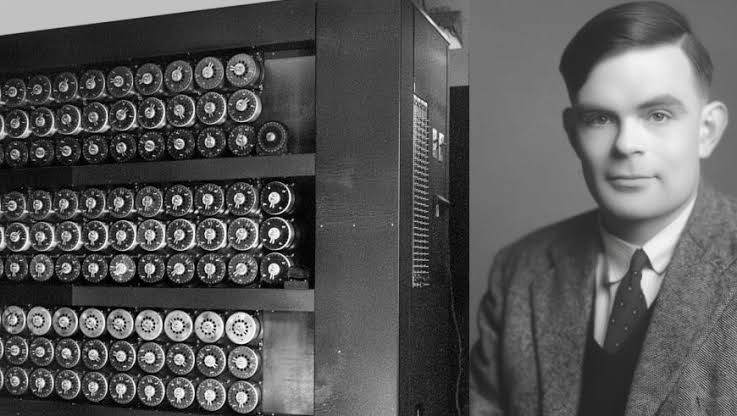
\includegraphics[width=0.6\textwidth]{img/alanturing_turingtest}
\caption{Alan Turing y su maquina christopher.}
\label{fig:turing}
\end{figure}

El objetivo de esta tarea es presentar, de forma ordenada y con mis propias palabras, cómo evolucionó la IA desde esas primeras ideas hasta la actualidad. Para ello, parto de la lectura de ocho artículos académicos, cada uno de los cuales aporta una pieza distinta del rompecabezas. Unos se centran en los orígenes teóricos y en la figura de Turing \parencite{grosz_what_2012, abramson_descartes_2011, milkowski_turings_2022}; otros recorren la historia general de la disciplina \parencite{haenlein_brief_2019, buchanan_very_2005}; y algunos más analizan el paso del enfoque simbólico al aprendizaje a partir de datos y a las máquinas generadoras de contenido \parencite{zhang_turing_2023, natale_lovelace_2024, wuppuluri_compression_2020}.

Debido a que los artículos están en inglés y no cubren todos los temas por igual, también me apoyé en una investigación complementaria hecha en internet. De esta forma completé los huecos que las lecturas no tratan con detalle, como los llamados inviernos de la IA, el papel de los lenguajes de programación en cada época y el surgimiento reciente del TinyML.

El trabajo está organizado en cuatro secciones principales. La primera presenta el desarrollo cronológico de la IA, desde sus orígenes hasta la era actual, con una línea de tiempo que relaciona cada etapa con los lenguajes de programación que se usaban. La segunda analiza la transición que llevó la IA de los sistemas basados en reglas a los sistemas que aprenden de los datos, así como el paso hacia el Machine Learning en dispositivos pequeños. La tercera es una reflexión crítica sobre cómo la capacidad de cómputo actual hizo posible lo que antes era solo teoría. Finalmente, presento mis conclusiones personales.

\section{Desarrollo cronológico de la IA}

El desarrollo de la Inteligencia Artificial no ha sido un camino continuo y sin obstáculos. Al contrario, ha estado marcado por momentos de gran entusiasmo, seguidos de periodos de desilusión y falta de financiamiento, y de nuevos renacimientos impulsados por avances técnicos. En esta sección se recorren las etapas principales de esta historia, y al final se presenta una línea de tiempo técnica que las relaciona con los lenguajes de programación de cada época.

\subsection{Los orígenes: filosofía, ficción y la idea de la máquina pensante}

La idea de que las máquinas pudieran pensar o comportarse como seres vivos no surgió con la computadora moderna. Desde la antigüedad, la humanidad ha imaginado máquinas y autómatas capaces de realizar tareas asombrosas. En la filosofía, pensadores como Descartes y Leibniz reflexionaron sobre si era posible crear dispositivos mecánicos capaces de razonar \parencite{buchanan_very_2005}. Incluso la ciencia ficción, con autores como Julio Verne e Isaac Asimov, contribuyó a alimentar esta fantasía y a poner sobre la mesa preguntas sobre la naturaleza humana \parencite{buchanan_very_2005}.

Sin embargo, fue Alan Turing quien convirtió estas especulaciones en un problema de investigación concreto. En su famoso artículo de 1950, Turing no solo planteó el test que lleva su nombre, sino que defendió la idea de que las máquinas podían hacer mucho más que calcular números. También respondió a diversas objeciones sobre la posibilidad de que una máquina pensara, entre ellas la famosa objeción planteada por Ada Lovelace, quien afirmaba que las máquinas solo podían hacer aquello para lo que fueron programadas y, por tanto, jamás podrían originar algo nuevo \parencite{grosz_what_2012}. Turing no estuvo de acuerdo, y señaló que las máquinas podían tomar por sorpresa a sus propios creadores.

Más recientemente, investigadores han estudiado con profundidad las ideas de Turing. Por un lado, se ha mostrado que el test de Turing no es una simple forma de conductismo, corriente que reduce la mente a la conducta observable. Al analizar sus escritos, se encuentra que Turing conocía y probablemente se inspiró en una prueba del lenguaje propuesta por Descartes mucho antes, y que ambos buscaban lo mismo: determinar si algo tiene una mente a partir de su comportamiento \parencite{abramson_descartes_2011}. Por otro lado, se ha interpretado el test de Turing como un ejercicio de ingeniería conceptual: Turing no pretendía analizar lo que significa la palabra inteligencia, sino darle un nuevo sentido que pudiera aplicarse a las máquinas \parencite{milkowski_turings_2022}.

\subsection{La IA simbólica y su esplendor (1956--1974)}

La Inteligencia Artificial como campo de estudio formal nació en 1956, durante un taller de verano en el Dartmouth College, en Estados Unidos. Fue ahí donde el investigador John McCarthy acuñó el término Inteligencia Artificial para describir la ambición de crear máquinas capaces de simular la inteligencia humana \parencite{haenlein_brief_2019}. Este evento reunió a un grupo reducido de investigadores convencidos de que todo aspecto del aprendizaje o de cualquier otra característica de la inteligencia puede, en principio, describirse tan con precisión que una máquina podría simularlo.

Durante estos primeros años, la investigación estuvo dominada por un enfoque conocido como IA simbólica, también llamada IA clásica. Este enfoque partía de la idea de que la inteligencia consiste en manipular símbolos siguiendo reglas lógicas. Los programas se construían describiendo de forma explícita el conocimiento y las reglas que debían seguir \parencite{buchanan_very_2005}. Se lograron avances notables: programas capaces de demostrar teoremas matemáticos, de jugar al ajedrez o a las damas, de resolver problemas de lógica y de entender lenguaje natural en contextos muy limitados \parencite{buchanan_very_2005}.

\begin{figure}[h!]
\centering
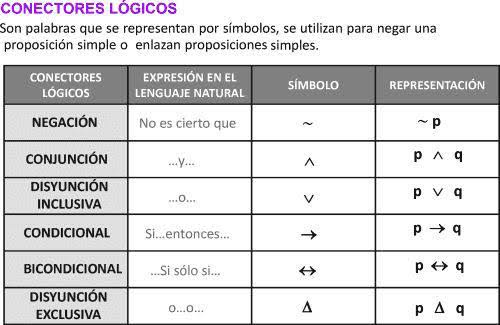
\includegraphics[width=0.6\textwidth]{img/ia_simbolica_lisp}
\caption{La IA simbólica (símbolos y reglas lógicas)}
\label{fig:simbolica}
\end{figure}

Una de las consecuencias de este enfoque fue el desarrollo de lenguajes de programación diseñados específicamente para manejar símbolos y reglas. El primero y más importante fue LISP, creado por John McCarthy en 1958. LISP se convirtió en el lenguaje preferido de la investigación en IA en Estados Unidos, y fue usado para escribir numerosos programas pioneros \parencite{buchanan_very_2005}. Poco después, en 1972, surgió en Europa el lenguaje Prolog, basado en la lógica, que resultó especialmente útil para construir sistemas capaces de razonar a partir de hechos y reglas.

\subsection{Los inviernos de la IA (1974--1980 y 1987--1993)}

A pesar del optimismo inicial, muy pronto quedó claro que la IA simbólica había sobreestimado la dificultad del problema. Las máquinas de la época eran demasiado lentas y tenían poca memoria, y los programas simbólicos no lograban resolver problemas del mundo real con la facilidad que se había prometido. Las expectativas habían sido tan altas que, cuando los resultados no llegaron, el interés y el financiamiento cayeron drásticamente.

Este primer periodo de desilusión, ocurrido entre 1974 y 1980, se conoce como el primer invierno de la IA. En 1973, el matemático James Lighthill publicó un informe crítico en el que concluía que la IA no estaba cumpliendo sus promesas, y esto llevó a una reducción significativa de los fondos destinados a la investigación en el Reino Unido y luego en Estados Unidos \parencite{haenlein_brief_2019}. Este dato, aunque no aparece con detalle en los artículos leídos, fue confirmado mediante investigación complementaria \parencite{ibm_history_ai, wikipedia_history_ai}.

No obstante, hubo un segundo renacimiento en los años ochenta, impulsado por los llamados sistemas expertos. La idea era capturar el conocimiento de un especialista humano y convertirlo en un conjunto de reglas que la computadora pudiera aplicar. Estos sistemas tuvieron cierto éxito comercial, y el campo volvió a atraer inversiones millonarias. Se crearon incluso computadoras especializadas, llamadas máquinas LISP, diseñadas para ejecutar este tipo de programas \parencite{buchanan_very_2005}.

Sin embargo, el entusiasmo volvió a derrumbarse hacia finales de los ochenta. Los sistemas expertos resultaron demasiado caros de mantener, difíciles de actualizar y muy limitados: solo funcionaban en terrenos muy acotados y fallaban ante cualquier situación inesperada. En esta época se generalizó el término invierno de la IA para describir el segundo colapso de financiamiento e interés, ocurrido entre finales de los ochenta y principios de los noventa \parencite{haenlein_brief_2019, ibm_history_ai}. Muchos investigadores, para evitar la asociación negativa del término, continuaron su trabajo bajo otros nombres: sistemas cognitivos, sistemas basados en conocimiento, razonamiento, entre otros \parencite{coursera_history_ai}.

\begin{figure}[h!]
\centering
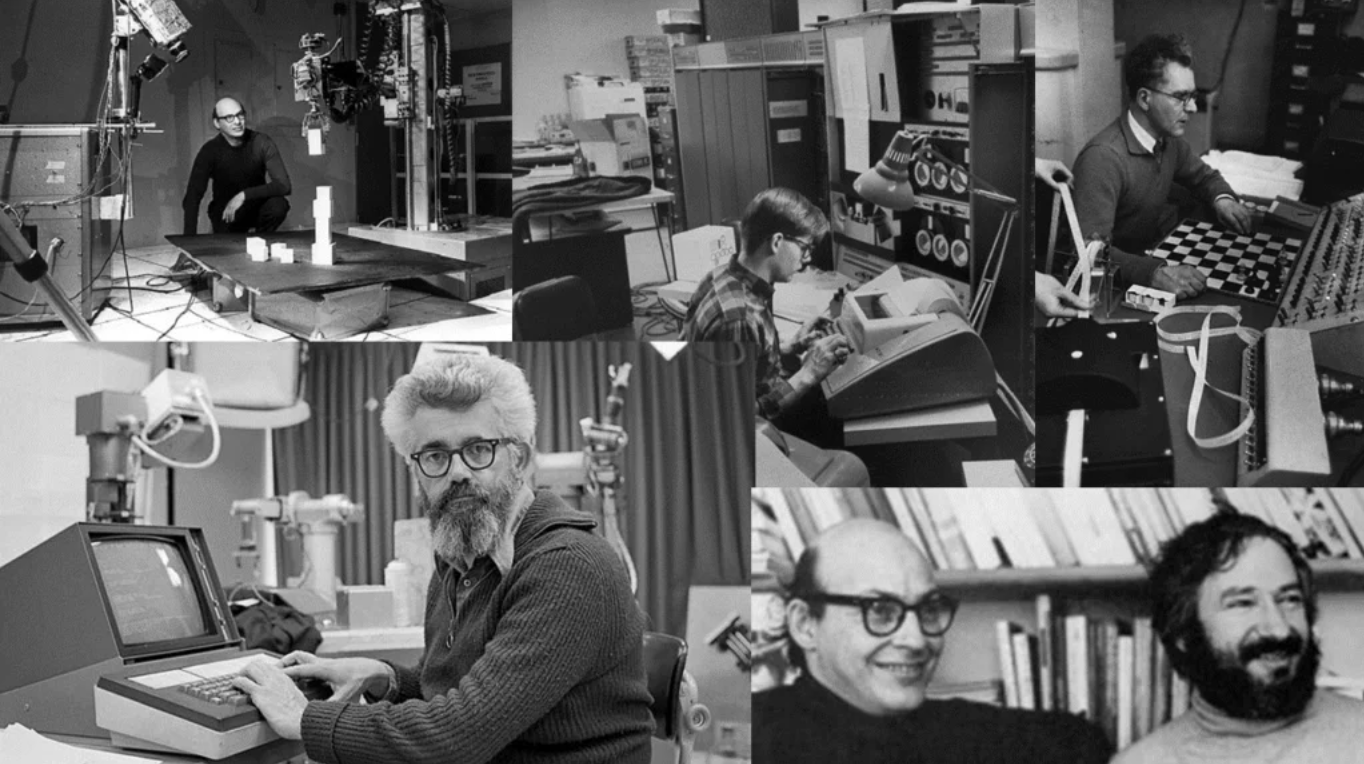
\includegraphics[width=0.6\textwidth]{img/inviernos_ia}
\caption{Los inviernos y renacimientos de la IA: picos y caídas del entusiasmo y la inversión.}
\label{fig:inviernos}
\end{figure}

\subsection{El auge del Machine Learning y la era del Big Data (1990--2017)}

Después de los inviernos de la IA, el campo tomó un nuevo rumbo. En lugar de intentar escribir a mano todas las reglas del conocimiento humano, los investigadores empezaron a crear programas capaces de \emph{aprender} a partir de datos. Nació así el Machine Learning, o Aprendizaje Automático, una área de la IA que crea programas que mejoran con la experiencia \parencite{haenlein_brief_2019}.

Este cambio de paradigma fue posible gracias a varios factores que coincidieron en el tiempo. En primer lugar, la aparición de grandes cantidades de datos, lo que se conoce como Big Data; en segundo lugar, el aumento del poder de cómputo, con computadoras cada vez más rápidas y baratas; y en tercer lugar, el uso de métodos matemáticos más sólidos \parencite{haenlein_brief_2019}. Durante los años noventa y la primera década del dos mil, el Machine Learning se aplicó con éxito a problemas como el reconocimiento de voz, el diagnóstico médico, la detección de fraudes y los sistemas de recomendación.

En paralelo, la evolución de las máquinas generadoras de contenido marcó otra línea importante dentro de esta historia. A partir de las ideas fundacionales de Turing, se desarrollaron primero modelos sencillos capaces de reproducir secuencias de datos, muy usados en el reconocimiento de voz; luego aparecieron las redes neuronales que pueden recordar información de pasos anteriores; y finalmente, con el auge del aprendizaje profundo, llegaron los grandes modelos de lenguaje como GPT, que hoy usamos en herramientas como ChatGPT para escribir, traducir o responder preguntas casi como una persona \parencite{zhang_turing_2023}.

En cuanto a los lenguajes de programación, durante esta etapa Python, creado por Guido van Rossum a principios de los años noventa, se convirtió en el lenguaje más usado en el Machine Learning y el aprendizaje profundo. Su forma de escribir código es sencilla y cuenta con muchas herramientas especializadas, como TensorFlow y Keras, lo que lo hizo la opción favorita de los investigadores \parencite{zhang_turing_2023}.

\subsection{Línea de tiempo técnica: avances y lenguajes predominantes}

La siguiente línea de tiempo resume la relación entre los hitos teóricos de la IA y los lenguajes de programación que predominaron en cada época.

\begin{figure}[H]
\centering
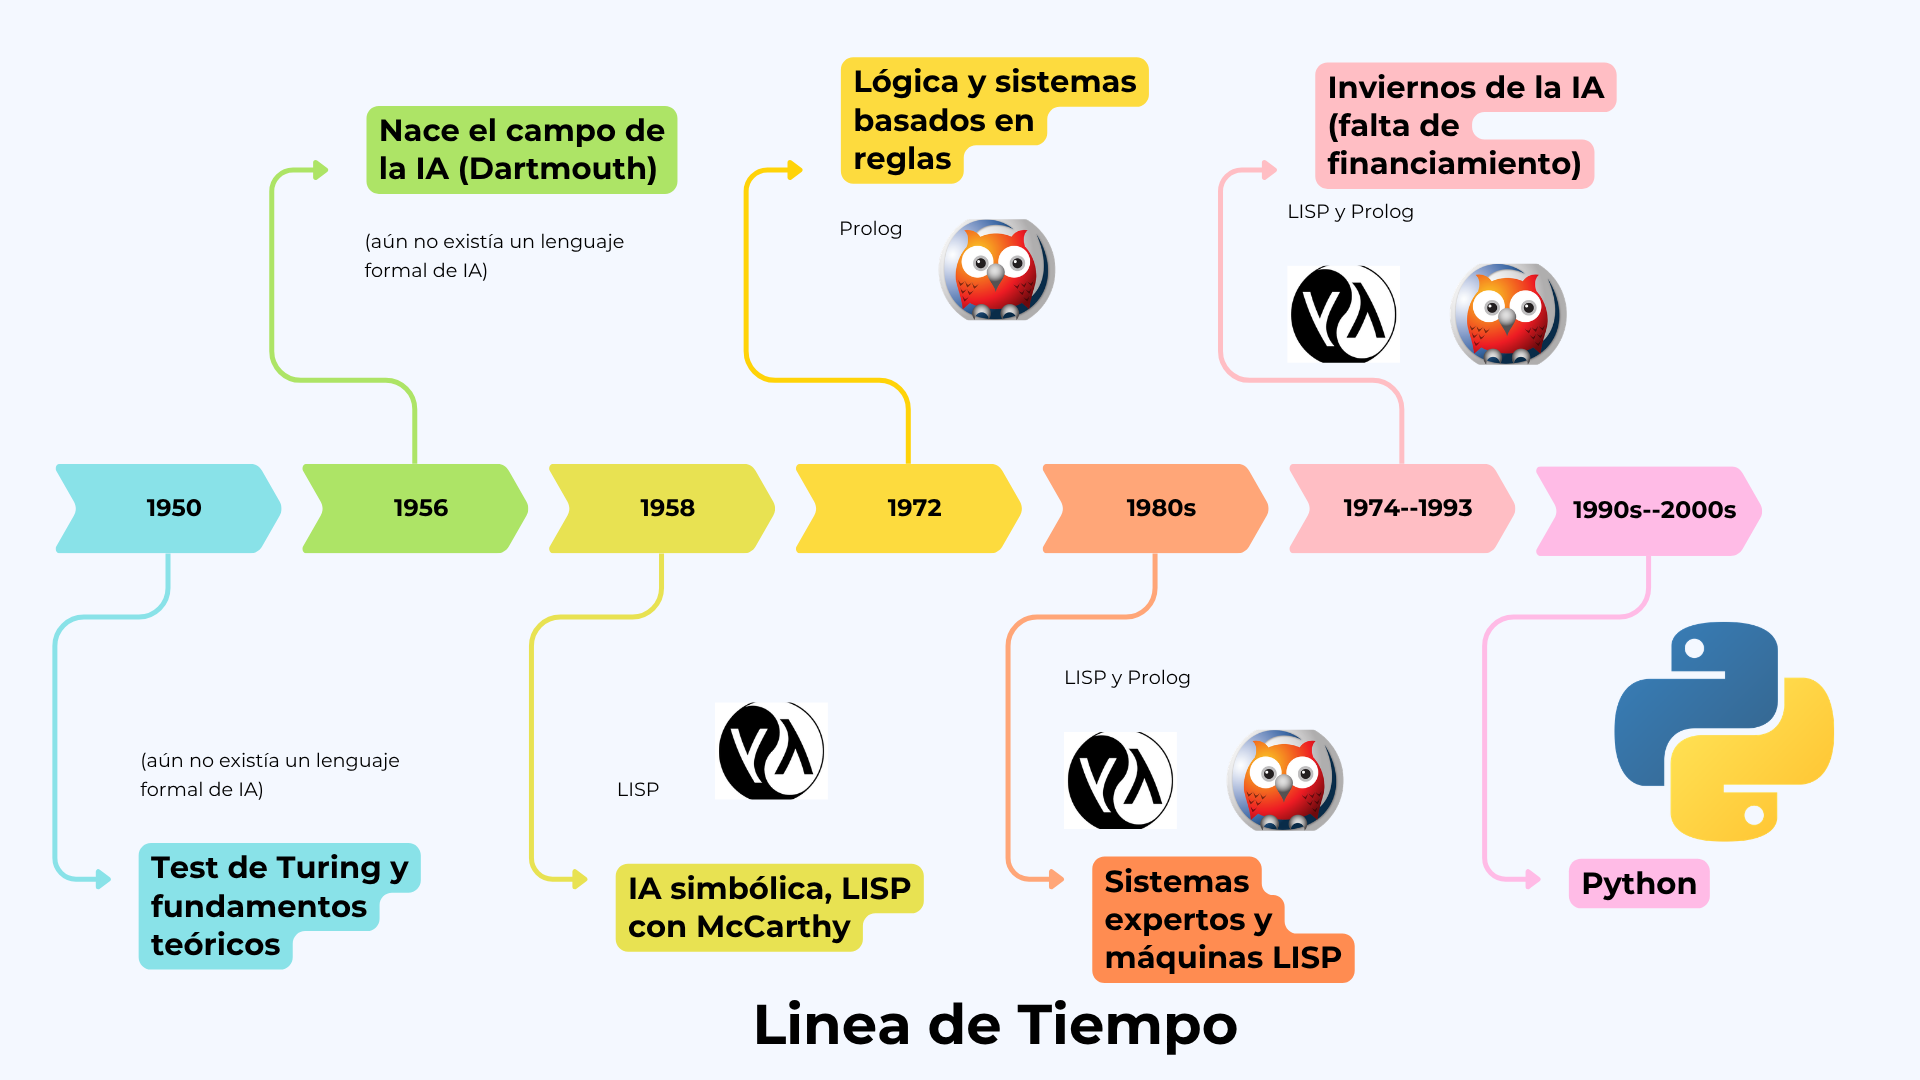
\includegraphics[width=0.8\textwidth]{img/linea_de_tiempo_tecnica}
\caption{Línea de tiempo técnica de la IA y sus lenguajes de programación.}
\label{fig:linea_tiempo}
\end{figure}

Como se observa, cada enfoque de la IA estuvo acompañado del lenguaje que mejor se adaptaba a sus necesidades. LISP destacó por su capacidad de manipular símbolos y listas; Prolog por su facilidad para representar reglas lógicas; y Python por su flexibilidad y su enorme ecosistema de bibliotecas que facilitan el trabajo con datos y redes neuronales.

\begin{figure}[H]
\centering
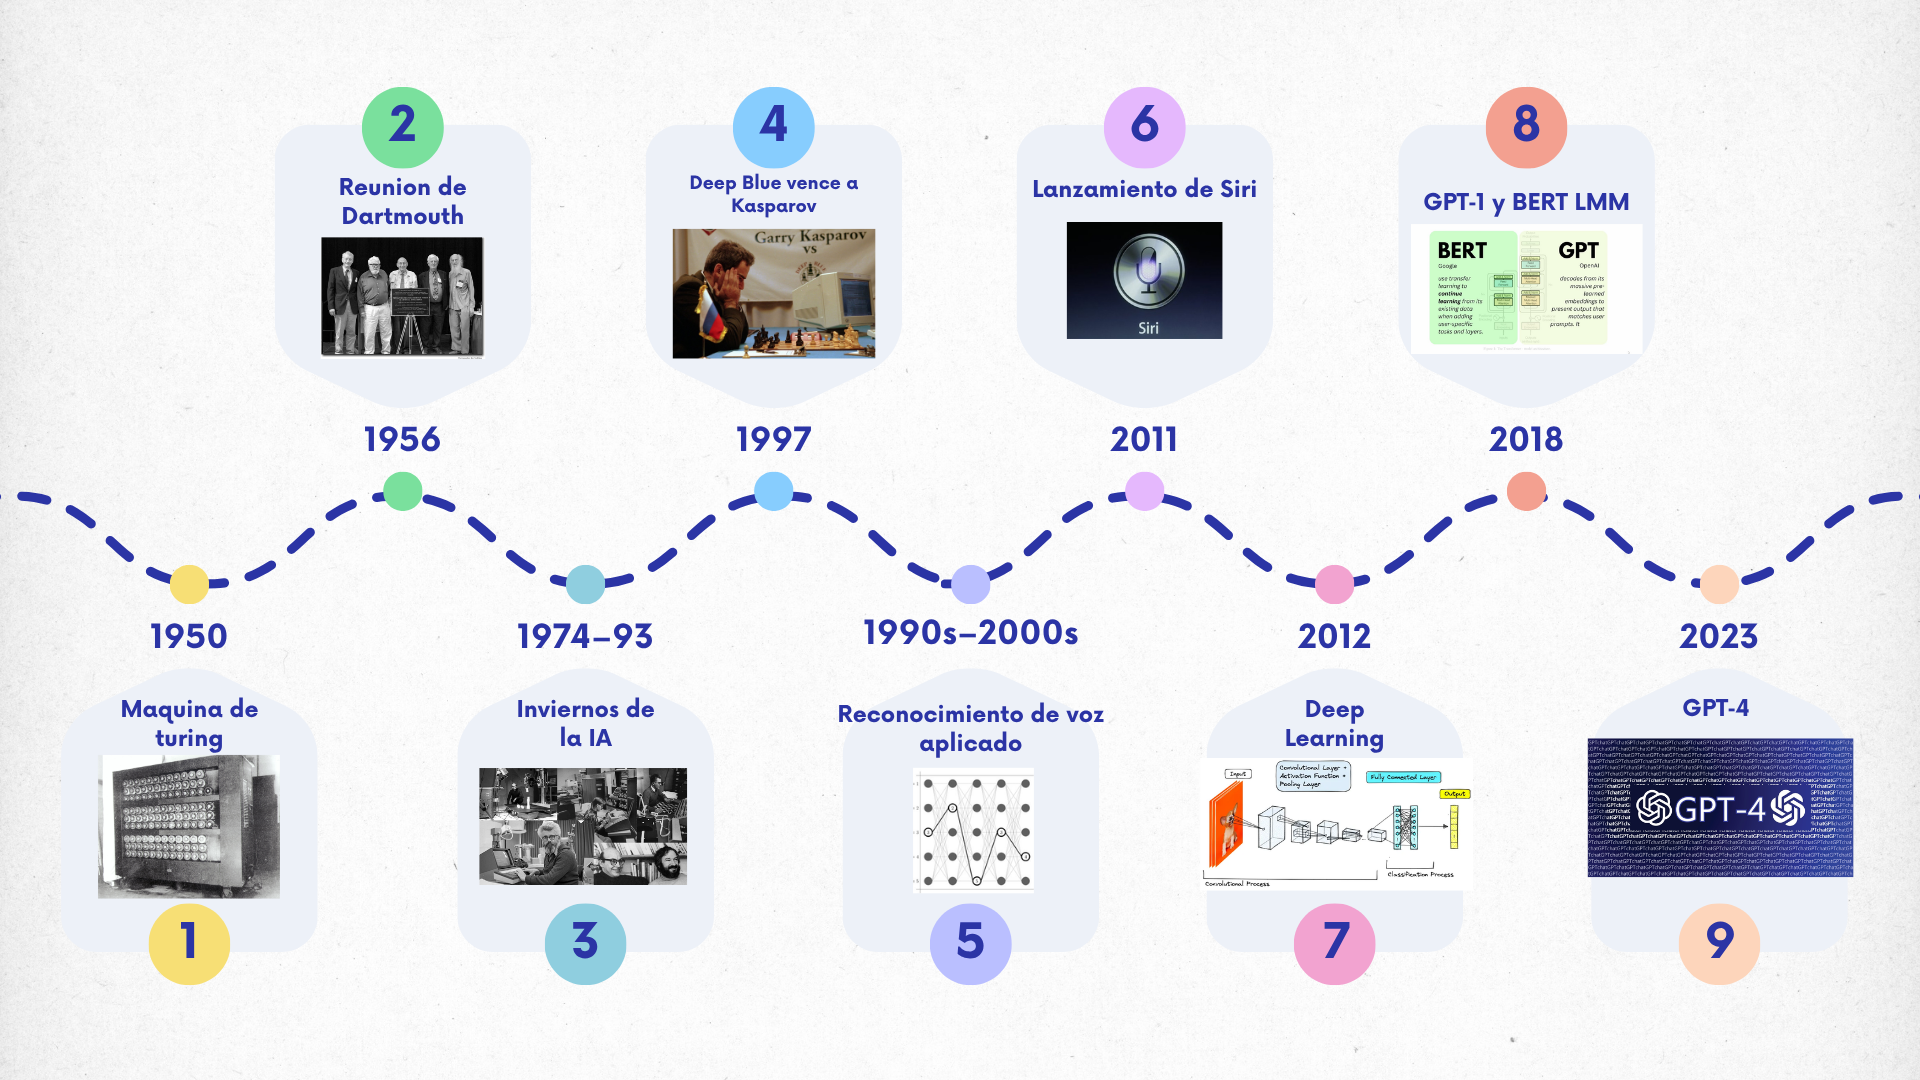
\includegraphics[width=0.95\textwidth]{img/linea_de_tiempo_final}
\caption{Línea de tiempo de los desarrollos de la IA, desde el test de Turing hasta los modelos generativos actuales.}
\label{fig:linea_final}
\end{figure}

\section{Análisis de la transición hacia el Machine Learning y TinyML}

\subsection{De los sistemas basados en reglas a los sistemas basados en datos}

La transición más importante en la historia de la IA fue el paso de los sistemas basados en reglas a los sistemas basados en datos. En la IA simbólica, el programador escribía a mano las reglas y el conocimiento; la computadora solo aplicaba esas reglas para obtener una respuesta. Este enfoque funcionaba en situaciones muy controladas, pero fallaba en el mundo real, donde el conocimiento es enorme, cambiante y difícil de explicar con reglas exactas \parencite{buchanan_very_2005}.

Con el Machine Learning el enfoque cambió por completo. En lugar de programar las reglas, el sistema aprende a descubrirlas a partir de ejemplos. Se le presentan miles o millones de datos con sus respuestas correctas, y el sistema va ajustando poco a poco su funcionamiento hasta que logra acertar también en datos que nunca había visto \parencite{zhang_turing_2023}. Este principio, que podríamos resumir como aprender de la experiencia, es lo que hizo posible el gran avance de la IA en las últimas décadas.

\subsection{El auge de las redes profundas y los modelos generativos}

Dentro de esta nueva etapa, el aprendizaje profundo, o Deep Learning, marcó un punto de inflexión. Se trata de redes neuronales con muchas capas, que aprenden poco a poco a reconocer cada vez más detalles en los datos. Hacia el año 2012, un programa llamado AlexNet ganó un importante concurso de reconocimiento de imágenes con mucho menos margen de error que el resto, y desde entonces este enfoque se convirtió en la tecnología dominante de la IA \parencite{zhang_turing_2023}.

\begin{figure}[h!]
\centering
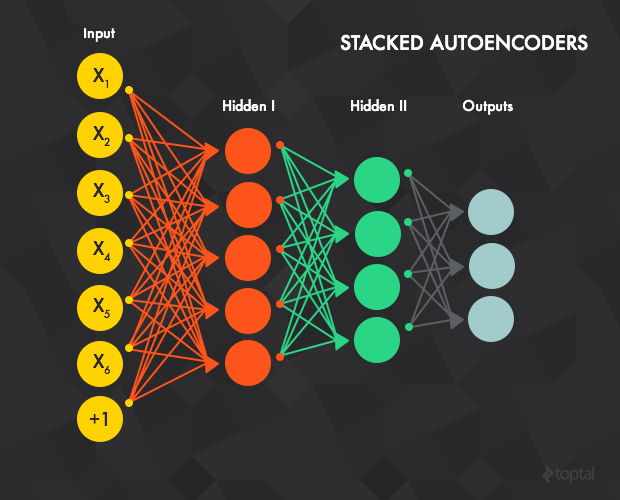
\includegraphics[width=0.6\textwidth]{img/deeplearning_redes}
\caption{Una red neuronal profunda (Deep Learning) con varias capas de neuronas.}
\label{fig:deeplearning}
\end{figure}

Este mismo impulso llevó al desarrollo de las máquinas generadoras de contenido, capaces de crear texto, imágenes o sonido. El paso de las redes simples a las arquitecturas más modernas permitió manejar textos largos y relacionar palabras muy distantes entre sí, lo que dio lugar a los grandes modelos de lenguaje como GPT y ChatGPT \parencite{zhang_turing_2023}. Estos modelos no solo entienden el lenguaje, sino que pueden generar respuestas, traducir, redactar código y hasta crear poesía, casi de forma indistinguible de una persona.

Desde una perspectiva más sencilla de entender, el investigador Héctor Zenil propuso una idea interesante: comprimir es comprender. Según este enfoque, una buena manera de explicar el mundo es encontrar pocos principios que expliquen mucha información, es decir, simplificar la realidad en una descripción corta. Esta idea conecta el éxito de la ciencia y de la computación con la capacidad de encontrar patrones simples detrás de fenómenos que parecen complicados \parencite{wuppuluri_compression_2020}. Esto ayuda a entender por qué los sistemas basados en datos han resultado tan poderosos: encuentran patrones y regularidades que al ojo humano se le escapan.

\subsection{El Machine Learning en dispositivos pequeños: TinyML}

El último eslabón de esta transición es el TinyML, es decir, la posibilidad de ejecutar programas de aprendizaje automático en dispositivos muy pequeños, baratos y que usan poca energía, como los microcontroladores que se usan en el Internet de las Cosas (IoT). Durante mucho tiempo, el Machine Learning se relacionó con poderosas computadoras en el centro de datos o la nube. Sin embargo, muchas aplicaciones necesitan tomar decisiones en el lugar, sin depender de una conexión a internet y sin consumir demasiada batería \parencite{zhang_turing_2023}.

\begin{figure}[h!]
\centering
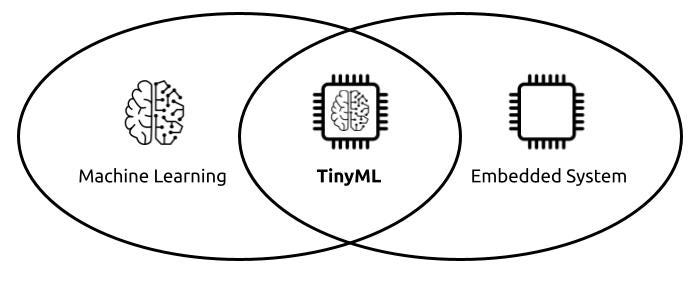
\includegraphics[width=0.6\textwidth]{img/tinyml_dispositivos}
\caption{TinyML: Machine Learning en microcontroladores o dispositivos de bajo consumo (Internet de las Cosas).}
\label{fig:tinyml}
\end{figure}

La información sobre TinyML se obtuvo mediante investigación complementaria, ya que ninguno de los artículos leídos la cubre directamente \parencite{survey_tinyml, tinyml_wikipedia}. Se trata de una tecnología reciente, surgida en la última década, que busca democratizar la IA llevándola a todo tipo de dispositivos pequeños. Para lograrlo, es necesario hacer los programas más ligeros y sencillos para que quepan en muy poca memoria y funcionen con apenas un poco de energía, parecida a la de una pila de botón durante un año \parencite{survey_tinyml}.

Ejemplos de aplicaciones de TinyML incluyen dispositivos de salud que detectan caídas o ritmos cardíacos anormales en tiempo real, sensores de agricultura que analizan el clima y el suelo, y asistentes de voz que responden sin necesidad de conectarse a la nube \parencite{tinyml_wikipedia}. La ventaja principal es la respuesta casi inmediata, la privacidad (los datos no salen del dispositivo) y el bajo consumo de energía. A cambio, hay que sacrificar parte de la precisión y de lo complejos que pueden ser los programas, ya que los microcontroladores tienen muy poca memoria y capacidad de cómputo \parencite{survey_tinyml}.

\section{Análisis crítico: la capacidad de cómputo como habilitador del Deep Learning}

Uno de los aprendizajes más interesantes de esta revisión es que las redes neuronales profundas no son una idea nueva. De hecho, las bases teóricas de las redes neuronales y del método para entrenarlas (conocido como retropropagación) ya existían desde las décadas de los sesenta y ochenta. Sin embargo, durante años estas ideas permanecieron casi olvidadas o fueron consideradas poco útiles, porque la tecnología de la época no podía ponerlas en práctica \parencite{zhang_turing_2023}.

La razón es sencilla: las redes neuronales profundas necesitan una cantidad enorme de cálculos y de datos para entrenarse. En los años ochenta y noventa, las computadoras eran demasiado lentas y tenían poca memoria, y no existían conjuntos de datos suficientemente grandes. Un investigador que quisiera entrenar una red neuronal profunda tendría que esperar días o semanas, incluso para tareas sencillas, lo que hacía el proceso poco práctico \parencite{haenlein_brief_2019}.

El cambio llegó por la combinación de tres factores. Primero, el aumento enorme de la capacidad de cómputo, impulsado en gran parte por el uso de tarjetas gráficas (GPU) y, más recientemente, de procesadores especializados, capaces de hacer muchísimas operaciones a la vez. Segundo, la disponibilidad de grandes cantidades de datos gracias a internet y al Big Data. Y tercero, la mejora de los algoritmos de entrenamiento \parencite{zhang_turing_2023}.

Este análisis permite entender por qué la IA generativa, que hoy parece algo cotidiano, fue imposible durante tanto tiempo. La idea de los grandes modelos de lenguaje existe desde hace años, pero solo con la potencia de cómputo y los datos masivos actuales pudo entrenarse un modelo con cientos de miles de millones de datos internos. La teoría estaba lista, pero la práctica necesitaba que la tecnología la alcanzara. Esto muestra que el avance de la IA no depende solo de las ideas, sino también de las máquinas que hacen posible llevarlas a la práctica \parencite{zhang_turing_2023}.

\section{Conclusiones personales}

Esta lectura analítica me permitió comprender que la Inteligencia Artificial no es un fenómeno reciente, sino el resultado de décadas de esfuerzo, fracasos y reinvención. Antes pensaba que la IA había surgido de la nada con herramientas como ChatGPT; ahora entiendo que su historia comienza con las preguntas de Alan Turing sobre las máquinas pensantes \parencite{grosz_what_2012}.    

Tres ideas me llamaron la atención en particular. Primero, que el test de Turing \parencite{milkowski_turings_2022, abramson_descartes_2011}. Segundo, que la historia de las redes neuronales profundas muestra que una buena idea no basta sin la tecnología que la haga viable: la teoría existía desde hacía décadas, pero el hardware necesitó alcanzarla \parencite{zhang_turing_2023}. Y tercero, que la creatividad que percibimos en las máquinas tiene mucho que ver con nuestra propia interpretación, no solo con lo que la máquina realmente hace \parencite{natale_lovelace_2024, grosz_what_2012}. 

Como estudiante de ingeniería, la lección más valiosa es que el avance tecnológico es un proceso lento e inestable, lleno de ciclos de entusiasmo y desilusión. Comprender esto me anima a no dejarme llevar solo por la novedad, sino a fundamentar lo que aprendo y a ser consciente tanto del potencial como de las limitaciones de esta tecnología \parencite{haenlein_brief_2019}.

\printbibliography[heading=bibintoc]

\appendix
\section{Anexo: Resumen escrito a mano}

Las siguientes imágenes corresponden al resumen elaborado a mano en mi libreta, de acuerdo con lo solicitado en la actividad.

\begin{figure}[H]
\centering
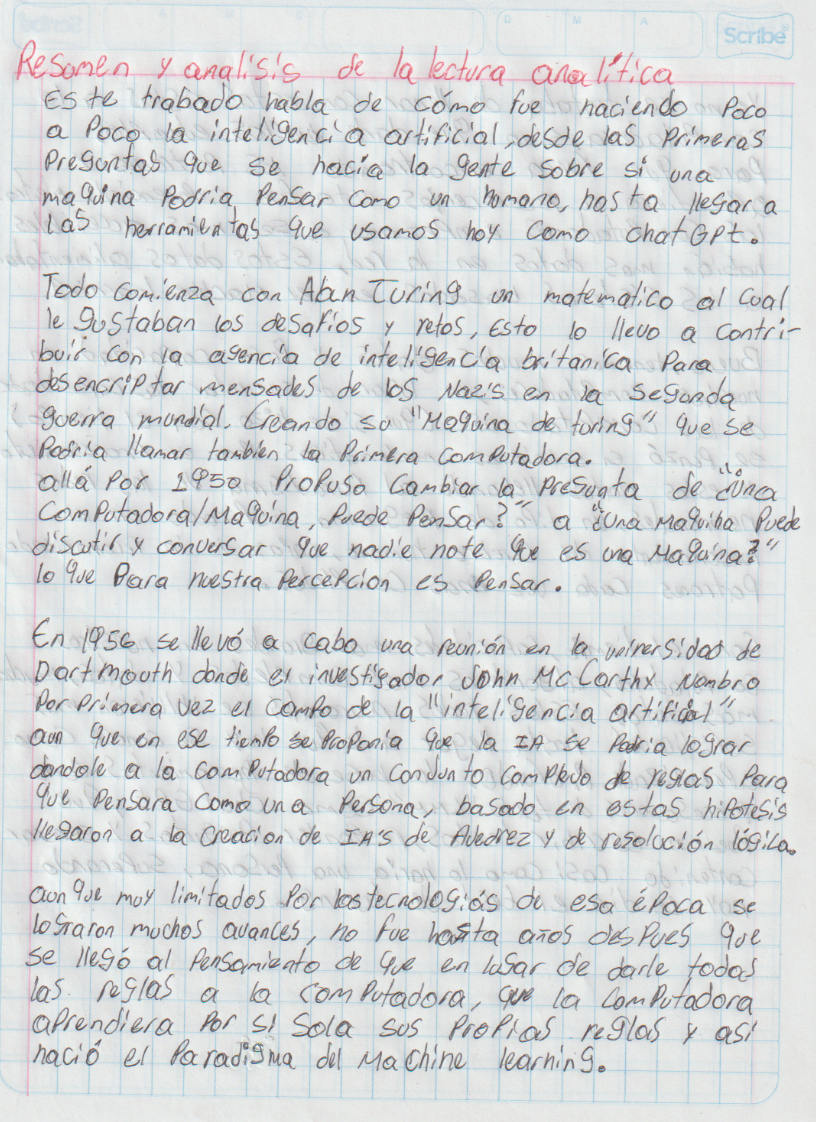
\includegraphics[width=\linewidth,height=0.7\textheight,keepaspectratio]{img/1_resumen}
\caption{Resumen escrito a mano, cuartilla 1 de 2.}
\label{fig:resumen1}
\end{figure}

\begin{figure}[H]
\centering
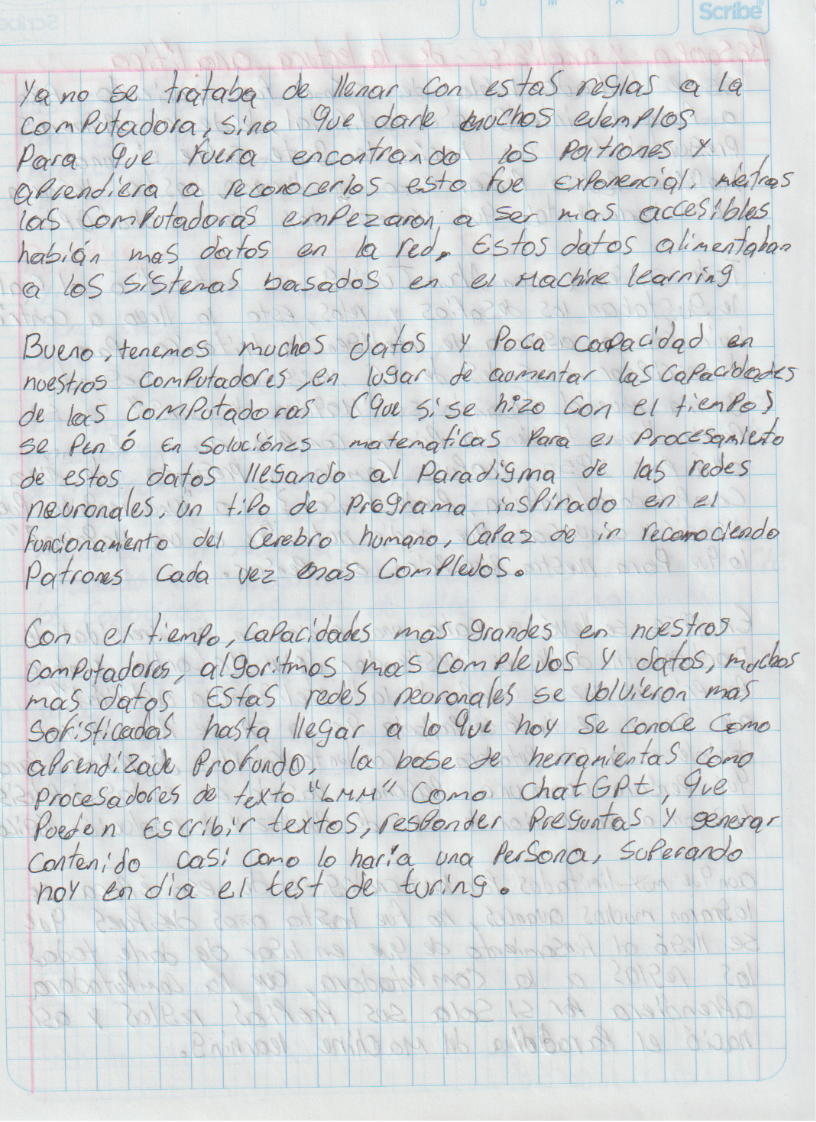
\includegraphics[width=\linewidth,height=0.7\textheight,keepaspectratio]{img/2_resumen}
\caption{Resumen escrito a mano, cuartilla 2 de 2.}
\label{fig:resumen2}
\end{figure}

\end{document}